\documentclass[11pt,letterpaper]{article}
\usepackage[margin=2.5cm]{geometry}
\usepackage[utf8]{inputenc}
\usepackage[T1]{fontenc}
\usepackage{lmodern}
\usepackage{amsmath,amssymb,amsthm,mathtools,bm}
\usepackage{enumitem}
\usepackage{booktabs}
\usepackage{tikz}
\usetikzlibrary{arrows.meta,patterns,positioning,calc}
\usepackage{pgfplots}
\pgfplotsset{compat=1.16}
\usepackage{titlesec}
\usepackage[hidelinks]{hyperref}

\setlength{\parindent}{0pt}
\setlength{\parskip}{0.5em}
\titleformat{\section}{\large\bfseries}{\thesection.}{0.6em}{}
\titleformat{\subsection}{\normalsize\bfseries}{\thesubsection.}{0.6em}{}

\theoremstyle{definition}
\newtheorem{definition}{Definition}[section]
\newtheorem{example}{Example}[section]
\newtheorem{exercise}{Exercise}[section]
\newtheorem{theorem}{Theorem}[section]
\newtheorem{remark}{Remark}[section]

\newcommand{\R}{\mathbb{R}}
\newcommand{\N}{\mathbb{N}}
\newcommand{\Z}{\mathbb{Z}}
\newcommand{\U}{\mathcal{U}}
\newcommand{\E}{\mathbb{E}}
\newcommand{\Var}{\operatorname{Var}}
\newcommand{\Cov}{\operatorname{Cov}}
\newcommand{\Normal}{\mathcal{N}}
\newcommand{\dd}{\,\mathrm{d}}
\newcommand{\T}{^{\top}}
\renewcommand{\P}{P}
\newcommand{\set}[1]{\left\{#1\right\}}
\newcommand{\given}{\mid}
\newcommand{\note}[1]{\textit{#1}}

\title{Lecture 2: Probability}
\author{}\date{}

\begin{document}
\maketitle

%=====================================================
\section{Sample space}

\begin{definition}[Sample space]
The \emph{sample space} $\Omega$ is the set of possible outcomes of an experiment.
\end{definition}

Below, $C$ denotes heads (\emph{cara}) and $S$ denotes tails (\emph{sello}).

\begin{example}
The set of possible outcomes of a coin toss: $\Omega = \set{\text{Cara}, \text{Sello}} = \set{C, S}$.
\end{example}
\begin{example}
Sample space of the toss of 2 coins: $\Omega = \set{CC, CS, SC, SS}$.
\end{example}
\begin{example}
Sample space of a die throw: $\Omega = \set{1,2,3,4,5,6}$.
\end{example}

\begin{definition}[Event]
Subsets of $\Omega$ are called \emph{events}.
\end{definition}

\begin{example}
Let $\Omega = \set{1,2,3,4,5,6}$ be the sample space of a die throw. Then $A = \set{1,2,3} \subset \Omega$ is the event of a die throw resulting in less than $4$.
\end{example}
\begin{example}
The event of the first coin of a two-coin throw resulting in heads: with $\Omega = \set{CC, CS, SC, SS}$,
\[
A = \set{CC, CS} \subset \Omega.
\]
\end{example}

%=====================================================
\section{Probability}
\begin{definition}[Probability]
A function $P$ that assigns a real number $P(A)$ to each event $A$ is a \emph{probability distribution} or a \emph{probability measure} if it satisfies the following axioms:
\begin{description}
\item[Axiom 1:] $P(A) \ge 0$ for every event $A$.
\item[Axiom 2:] $P(\Omega) = 1$.
\item[Axiom 3:] If $A_1, A_2, \dots$ are disjoint, that is, $A_i \cap A_j = \emptyset$ for $i \ne j$, then
\[
P(A_1 \cup A_2 \cup A_3 \cup \cdots) = \sum_{i=1}^{\infty} P(A_i),
\qquad\text{i.e.}\qquad
P\Big(\bigcup_{i=1}^{\infty} A_i\Big) = \sum_{i=1}^{\infty} P(A_i).
\]
\end{description}
\end{definition}

\paragraph{What does the probability of an event happening mean?}
There are several interpretations:
\begin{enumerate}[label=(\roman*)]
\item \textbf{Frequentist:} the probability $P(A)$ of an event happening is the proportion of times an event $A$ occurs after repeating the same experiment many times under identical conditions.
\item \textbf{Degrees of belief:} probability here is a measure of how much an observer is convinced that an event $A$ is true or will occur.
\item \textbf{Extension of logic for reasoning under uncertainty:} logic tells whether certain propositions are true or false. Probability quantifies how plausible a proposition is given available information. That is, probability is a measure of our state of knowledge about a proposition, not a property of the physical world itself.
\end{enumerate}

\subsection{Other properties}
\begin{itemize}
\item $P(\emptyset) = 0$.
\item $A \subseteq B \Rightarrow P(A) \le P(B)$.

If $A \subseteq B$, then we can come up with a partition of $B$ such as
\[
B = A \cup (B - A) = A \cup (B \cap A^c).
\]
Since $A$ and $B \cap A^c$ are disjoint, by Axiom 3
\[
P(B) = P\big(A \cup (B \cap A^c)\big) = \new{P(A) + P(B \cap A^c)} \ge P(A),
\]
because $P(B \cap A^c) \ge 0$.
\item If $B = \Omega$: $0 \le P(A) \le P(\Omega) = 1$, so $0 \le P(A) \le 1$.
\item Since $\Omega = A \cup A^c$: $P(\Omega) = P(A \cup A^c) = P(A) + P(A^c) = 1$, so
\[
P(A^c) = 1 - P(A).
\]
\end{itemize}

\begin{exercise}
Let $A$ and $B$ be two non-disjoint sets (this is, $A \cap B \neq \emptyset$). Show that the sets $A \cap B^c$, $A \cap B$ and $A^c \cap B$ are disjoint between each other.

\emph{Solution.}
\begin{align*}
(A \cap B^c) \cap (A \cap B) &= (A \cap A) \cap (B^c \cap B) = A \cap \emptyset = \emptyset,\\
(A \cap B^c) \cap (A^c \cap B) &= (A \cap A^c) \cap (B^c \cap B) = \emptyset \cap \emptyset = \emptyset,\\
(A \cap B) \cap (A^c \cap B) &= (A \cap A^c) \cap (B \cap B) = \emptyset \cap B = \emptyset,
\end{align*}
where $A \cap \emptyset = \set{x \mid x \in A \wedge x \in \emptyset} = \emptyset$, since $x \in \emptyset$ is false.
Moreover, their union is $A \cup B$:
\begin{align*}
\big[(A \cap B^c) \cup (A \cap B)\big] \cup (A^c \cap B)
&= \big[A \cap \new{(B^c \cup B)}\big] \cup (A^c \cap B)
= (A \cap \new{\U}) \cup (A^c \cap B)\\
&= \new{A} \cup (A^c \cap B) = \new{(A \cup A^c) \cap (A \cup B)} = \new{\U} \cap (A \cup B) = A \cup B.
\end{align*}
\end{exercise}

\paragraph{$P(A \cup B)$ when $A \cap B \neq \emptyset$.}
Using the disjoint decomposition above,
\begin{align*}
P(A \cup B) &= P\big[(A \cap B^c) \cup (A \cap B) \cup (A^c \cap B)\big]\\
&= P(A \cap B^c) + P(A \cap B) + P(A^c \cap B) \new{{}+ P(A \cap B) - P(A \cap B)}\\
&= \new{P\big((A \cap B^c) \cup (A \cap B)\big)} + \new{P\big((A^c \cap B) \cup (A \cap B)\big)} - P(A \cap B).
\end{align*}
Since $(A^c \cap B) \cup (A \cap B) = (B \cap A^c) \cup (B \cap A) = B \cap (A^c \cup A) = B$, and similarly $(A \cap B^c) \cup (A \cap B) = A$,
\[
P(A \cup B) = P(A) + P(B) - P(A \cap B).
\]

\begin{exercise}
There are 4 candidates for president: $A$, $B$, $C$ and $D$. According to some survey, it was estimated that $A$ has a $20\%$ chance of winning the election, whereas $B$ has a $40\%$ chance of winning. What is the probability of the election being won by $A$ or $B$?
\end{exercise}

\begin{exercise}
In a residential area, $60\%$ of homes have internet service provided by the local cable company, $80\%$ have television service from the same company and $50\%$ have both services.\footnote{Devore, \emph{Probability and Statistics for Engineering and the Sciences}, Example 2.14.} If we randomly select one house:
\begin{enumerate}[label=(\roman*)]
\item What is the probability that the selected house has at least one of the services provided by the cable company?
\[
P(A \cup B) = P(A) + P(B) - P(A \cap B).
\]
\item What is the probability that the selected house has exactly one service? The event is
\[
\set{x \mid (x \in A \wedge x \notin B) \vee (x \notin A \wedge x \in B)} = (A \cap B^c) \cup (A^c \cap B),
\]
where $A - B = A \cap B^c$ and $B - A = B \cap A^c$. These two sets are disjoint, so
\[
P\big((A \cap B^c) \cup (A^c \cap B)\big) = P(A \cap B^c) + P(A^c \cap B).
\]
Since $A = A \cap \U = A \cap (B \cup B^c) = (A \cap B) \cup (A \cap B^c)$ and $B = (A \cap B) \cup (A^c \cap B)$,
\[
P(A) = P(A \cap B) + P(A \cap B^c), \qquad P(B) = P(A \cap B) + P(A^c \cap B),
\]
and therefore
\[
P\big((A \cap B^c) \cup (B \cap A^c)\big) = P(A) + P(B) - 2P(A \cap B).
\]
\begin{center}
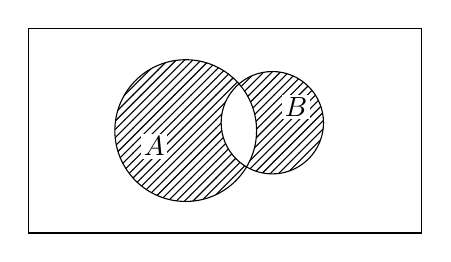
\begin{tikzpicture}
\draw (0,0) rectangle (5,2.6);
\begin{scope}[even odd rule]
\clip (2.0,1.3) circle (0.9) (3.1,1.4) circle (0.65);
\fill[pattern=north east lines] (0,0) rectangle (5,2.6);
\end{scope}
\draw (2.0,1.3) circle (0.9); \draw (3.1,1.4) circle (0.65);
\node[fill=white,inner sep=1pt] at (1.6,1.1) {$A$}; \node[fill=white,inner sep=1pt] at (3.4,1.6) {$B$};
\end{tikzpicture}
\end{center}
\end{enumerate}
\end{exercise}

\section{Probability on finite sample spaces}
Let us consider the sample space of a coin throw, $\Omega = \set{C, S}$. What is the probability of observing $C$? Concretely, if $A = \set{C}$ is the event of observing heads (cara), the question is: what is $P(A)$?

\paragraph{Principle of indifference.} There is no reason to think that an element of the sample set has distinct chances of occurring with respect to the other members of the set.

The sample space can be written as
\[
\Omega = \set{C, S} = \underbrace{\set{C}}_{A_1} \cup \underbrace{\set{S}}_{A_2},
\]
then
\[
P(\Omega) = P(A_1 \cup A_2) = \underbrace{P(A_1)}_{\new{p}} + \underbrace{P(A_2)}_{\new{p}} = 1.
\]
By the principle of indifference $P(A_1) = P(A_2) = p$, so $2p = 1 \Rightarrow p = \tfrac12$.

In general, for a sample space $\Omega = \set{\omega_1, \omega_2, \dots, \omega_n}$ we can write
\[
\Omega = \set{\omega_1} \cup \set{\omega_2} \cup \cdots \cup \set{\omega_n},
\]
then
\[
P(\Omega) = \sum_{i=1}^{n} P(\set{\omega_i}) = 1.
\]
Because of the indifference principle, $P(\set{\omega_i}) = \theta$ for all $i$, so
\[
\sum_{i=1}^{n} P(\set{\omega_i}) = \sum_{i=1}^{n} \new{\theta} = \new{\theta} \sum_{i=1}^{n} 1 = \theta\, \new{n} = 1
\ \Rightarrow\ \theta = \frac{1}{n},
\qquad
P(\set{\omega_i}) = \frac1n = \frac{1}{|\Omega|}.
\]

We can also have an event with more than one element, e.g.\ $A = \set{\omega_1, \dots, \omega_{|A|}}$. Then we can split it as $A = \set{\omega_1} \cup \cdots \cup \set{\omega_{|A|}}$ and
\[
P(A) = \sum_{i=1}^{|A|} \underbrace{P(\set{\omega_i})}_{1/|\Omega|} = \frac{1}{|\Omega|} \sum_{i=1}^{|A|} 1 = \frac{|A|}{|\Omega|}.
\]


The probability $P(A) = \dfrac{|A|}{|\Omega|}$ is called the \emph{uniform probability distribution}.

\begin{example}
What is the probability of getting a value less than $4$ in a die throw? With $\Omega = \set{1,2,3,4,5,6}$ and $A = \set{1,2,3}$,
\[
P(A) = \frac{|A|}{|\Omega|} = \frac{3}{6} = \frac12.
\]
\end{example}

\begin{example}
In a two-dice throw, what is the probability of a result summing up to $5$? Writing $D_1$ and $D_2$ for the results of each die,
\[
P(D_1 + D_2 = 5) = \frac{4}{36} = \frac19.
\]
\end{example}

\subsection{Counting techniques}
An ordered subset is called a \emph{permutation}. The number of permutations of size $k$ that can be formed out of $n$ objects is
\[
P_{k,n} = \frac{n!}{(n-k)!}.
\]
An unordered subset is called a \emph{combination}. The number of combinations of size $k$ out of $n$ objects is
\[
C_{k,n} = \binom{n}{k} = \frac{n!}{k!\,(n-k)!}.
\]

\begin{example}[Example 2.23, Devore]
$n = 25$, $k = 6$, where the $25$ objects are split into two groups, $l$ (with $10$ objects) and $i$ (with $15$).\footnote{Devore, \emph{Probability and Statistics for Engineering and the Sciences}, Example 2.23.} The probability of choosing $3$ from each group is
\[
P(l = 3, i = 3) =\frac{\binom{10}{3}\binom{15}{3}}{\binom{25}{6}}.
\]
\end{example}

%=====================================================
\section{Independent events}
Two events $A$ and $B$ are \emph{independent} if
\[
P(A \cap B) = P(A)\,P(B).
\]
This is denoted as $A \perp B$.

Three events $A$, $B$ and $C$ are independent if
\[
P(A \cap B \cap C) = P(A)\,P(B)\,P(C).
\]
For this to happen we also need
\[
P(A \cap B) = P(A)P(B), \qquad P(A \cap C) = P(A)P(C), \qquad P(B \cap C) = P(B)P(C).
\]
In general, a set of events $\set{A_i : i \in I}$ is independent if
\[
P\Big(\bigcap_{i \in J} A_i\Big) = \prod_{i \in J} P(A_i)
\]
for every finite subset $J$ of $I$.

\begin{example}
Toss a coin $10$ times. Let $A$ = ``at least one head''.\footnote{Wasserman, \emph{All of Statistics}, Example 1.10.} Let $T_j$ be the event that tails occurs on the $j$-th toss. We can state $A$ as
\[
A:\ \#\text{heads} \ge 1, \qquad A^c:\ \#\text{heads} < 1, \ \text{i.e.}\ \#\text{tails} = 10.
\]
Since $P(A \cup A^c) = P(A) + P(A^c) = 1$, we have $P(A) = 1 - P(A^c)$, with $A^c = T_1 \cap T_2 \cap \cdots \cap T_{10}$. Using independence,
\[
P(A) = 1 - P(T_1)\,P(T_2)\cdots P(T_{10}) = 1 - \frac{1}{2^{10}}.
\]
\end{example}

%=====================================================
\section{Conditional probability}
The \emph{conditional probability} of $A$ given that $B$ has occurred is defined as
\[
P(A \mid B) = \frac{P(A \cap B)}{P(B)},
\]
where $P(B) > 0$. Thus, for the uniform distribution,
\[
P(A \mid B) = \frac{|A \cap B|/|\Omega|}{|B|/|\Omega|} = \frac{|A \cap B|}{|B|}.
\]

$P(\cdot \mid B)$ satisfies all of the probability axioms:
\begin{enumerate}[label=(\roman*)]
\item $P(A \mid B) \ge 0$,
\item $P(\Omega \mid B) = 1$,
\item $P\big(\bigcup_{i=1}^{\infty} A_i \mid B\big) = \sum_{i=1}^{\infty} P(A_i \mid B)$ for disjoint $A_1, A_2, \dots$
\end{enumerate}

\begin{example}
A container stores $5$ defective transistors (that fail immediately), $10$ partially defective (that fail after a couple of hours) and $25$ acceptable. A transistor is chosen at random. If it doesn't immediately fail, what is the probability for the transistor to be acceptable?

Let $A$: defective, $B$: partially defective, $C$: acceptable. Then $A^c = C \cup B$ and
\[
P(C \mid A^c) = \frac{P(C \cap A^c)}{P(A^c)} = \frac{|C \cap A^c|}{|A^c|} = \frac{|C \cap (C \cup B)|}{|C \cup B|}.
\]
Since
\begin{align*}
C \cap (C \cup B) &= \set{x \mid x \in C \wedge (x \in C \vee x \in B)}\\
&= \set{x \mid (x \in C \wedge x \in C) \vee \underbrace{(x \in C \wedge x \in B)}_{\text{false}}} = \set{x \mid x \in C} = C,
\end{align*}
we get
\[
P(C \mid A^c) = \frac{|C|}{|C \cup B|} = \frac{25}{35} = \frac57.
\]
\end{example}

\begin{example}
A medical test for disease $D$ has outcomes $+$ and $-$.\footnote{Wasserman, \emph{All of Statistics}, Example 1.13.} The probabilities are
\begin{center}
\begin{tabular}{c|cc}
 & $D$ & $D^c$\\ \hline
$+$ & $0.009$ & $0.099$\\
$-$ & $0.001$ & $0.891$
\end{tabular}
\end{center}
Find the probability of testing $+$ given $D$:
\[
P(+ \mid D) = \frac{P(+ \cap D)}{P(D)} = \frac{0.009}{0.01} = \frac{9\times10^{-3}}{1\times10^{-2}} = 0.9.
\]
Similarly,
\[
P(- \mid D^c) = \frac{P(- \cap D^c)}{P(D^c)} = \frac{0.891}{0.99} = 0.9.
\]
Probability of having the disease given that a test resulted positive:
\[
P(D \mid +) = \frac{0.009}{0.009 + 0.099} \approx 0.083.
\]
\end{example}

If $A \perp B$, then
\[
P(A \mid B) = \frac{P(A \cap B)}{P(B)} = \frac{P(A)\,P(B)}{P(B)} = P(A).
\]

\begin{homework}{2}
A study of gas stations in the Biob\'io Region looked at three characteristics of their customers:
\begin{align*}
A &= \set{\text{the car is from the latest model year}},\\
B &= \set{\text{the car runs on diesel}},\\
C &= \set{\text{the customer pays with a credit card}},
\end{align*}
with
\begin{gather*}
P(A) = 0.17,\quad P(B) = 0.10,\quad P(C) = 0.36,\\
P(A \cap B) = 0.06,\quad P(A \cap C) = 0.08,\quad P(B \cap C) = 0.03.
\end{gather*}
Also, $52\%$ of the customers have none of the three characteristics. For a customer chosen at random, find:
\begin{enumerate}[label=(\roman*)]
\item the probability that the car is not from the latest year and the customer does not pay by credit card;
\item the probability that the car does not run on diesel and the customer pays by credit card;
\item whether $A$ and $C$ are independent;
\item given that the car is from the latest year, the probability that it runs on diesel;
\item given that the customer does not pay by credit card, the probability that the car is from the latest year and does not run on diesel.
\end{enumerate}

\soln
``None of the three'' is $A^c \cap B^c \cap C^c = (A \cup B \cup C)^c$, so $P(A \cup B \cup C) = 1 - 0.52 = 0.48$. Inclusion--exclusion for three events gives the one probability we are missing:
\begin{align*}
P(A \cup B \cup C) &= P(A) + P(B) + P(C) - P(A \cap B) - P(A \cap C) - P(B \cap C) + P(A \cap B \cap C),\\
0.48 &= \new{0.46} + P(A \cap B \cap C)
\quad\Longrightarrow\quad \new{P(A \cap B \cap C) = 0.02}.
\end{align*}
\begin{enumerate}[label=(\roman*)]
\item By De Morgan, $A^c \cap C^c = (A \cup C)^c$:
\[
P(A^c \cap C^c) = 1 - P(A \cup C) = 1 - \big[P(A) + P(C) - P(A \cap C)\big] = 1 - \new{0.45} = \new{0.55}.
\]
\item $C$ splits into the disjoint pieces $C \cap B$ and $C \cap B^c$, so
\[
P(B^c \cap C) = P(C) - P(B \cap C) = 0.36 - 0.03 = \new{0.33}.
\]
\item $P(A)\,P(C) = 0.17 \times 0.36 = \new{0.0612} \neq 0.08 = P(A \cap C)$, so $A$ and $C$ are \emph{not} independent.
\item $P(B \mid A) = \dfrac{P(A \cap B)}{P(A)} = \dfrac{0.06}{0.17} = \new{\dfrac{6}{17}} \approx 0.353$.
\item We need $P(A \cap B^c \mid C^c) = P(A \cap B^c \cap C^c)/P(C^c)$. Removing from $A$ the parts that lie in $B$ or in $C$, and adding back their overlap (removed twice),
\begin{align*}
P(A \cap B^c \cap C^c) &= P(A) - P(A \cap B) - P(A \cap C) + \new{P(A \cap B \cap C)}\\
&= 0.17 - 0.06 - 0.08 + \new{0.02} = \new{0.05},
\end{align*}
and $P(C^c) = 1 - 0.36 = 0.64$. Therefore
\[
P(A \cap B^c \mid C^c) = \frac{0.05}{0.64} = \new{\frac{5}{64}} \approx 0.078.
\]
\end{enumerate}
\end{homework}

%=====================================================
\section{Law of total probability}
Let $A_1, \dots, A_k$ be a partition of $\Omega$, i.e.\ $\Omega = A_1 \cup \cdots \cup A_k$ with $A_i \cap A_j = \emptyset$ for all $i \neq j$. For an event $B$ we have
\[
B = B \cap \Omega = B \cap (A_1 \cup \cdots \cup A_k) = (B \cap A_1) \cup (B \cap A_2) \cup \cdots \cup (B \cap A_k).
\]
These sets are disjoint, e.g.\ $(B \cap A_1) \cap (B \cap A_2) = B \cap B \cap \underbrace{A_1 \cap A_2}_{\emptyset} = B \cap \emptyset = \emptyset$. Therefore
\[
P(B) = \sum_{i=1}^{k} P(B \cap A_i) = \sum_{i=1}^{k} P(B \mid A_i)\,P(A_i).
\]

\begin{example}
There are $3$ bags, each one containing $100$ small balls:
\begin{enumerate}[label=(\roman*)]
\item Bag 1 contains $75$ red balls and $25$ blue balls.
\item Bag 2 contains $60$ red balls and $40$ blue balls.
\item Bag 3 contains $45$ red balls and $55$ blue balls.
\end{enumerate}
If I pick a bag randomly and then draw a ball from the chosen bag, what would be the probability of getting a red ball? Let $R$ be the event ``red ball'' and $B_i$ the event ``bag $i$ is chosen'', with $P(B_i) = 1/3$:
\begin{align*}
P(R) &= \sum_{i=1}^{3} P(R \cap B_i) = \sum_{i=1}^{3} P(R \mid B_i)\,P(B_i)
= \frac13\big[P(R \mid B_1) + P(R \mid B_2) + P(R \mid B_3)\big]\\
&= \frac13\left[\frac{75}{100} + \frac{60}{100} + \frac{45}{100}\right] = \frac13\left(\frac{180}{100}\right) = \frac{6}{10} = 0.6.
\end{align*}
\end{example}


\begin{homework}{2}
A box has two coins: a fair coin and a trick coin with heads on both sides. One coin is chosen at random, with equal probability, and tossed twice. Let
\[
A = \set{\text{first toss is heads}},\quad
B = \set{\text{second toss is heads}},\quad
C = \set{\text{the fair coin is chosen}}.
\]
Find $P(A \mid C)$, $P(B \mid C)$, $P(A \cap B \mid C)$, $P(A)$, $P(B)$ and $P(A \cap B)$. Are $A$ and $B$ \emph{conditionally} independent given $C$, that is, $P(A \cap B \mid C) = P(A \mid C)\,P(B \mid C)$? Are they \emph{marginally} independent, $P(A \cap B) = P(A)\,P(B)$?

\soln
With the fair coin the two tosses are independent:
\[
P(A \mid C) = P(B \mid C) = \frac12,
\qquad
P(A \cap B \mid C) = \frac12 \cdot \frac12 = \new{\frac14} = P(A \mid C)\,P(B \mid C).
\]
So $A$ and $B$ are conditionally independent given $C$. With the trick coin every toss is heads: $P(A \mid C^c) = P(B \mid C^c) = P(A \cap B \mid C^c) = 1$. By the law of total probability, with $P(C) = P(C^c) = \tfrac12$,
\begin{align*}
P(A) &= P(A \mid C)\,P(C) + P(A \mid C^c)\,P(C^c) = \new{\tfrac12}\cdot\tfrac12 + \new{1}\cdot\tfrac12 = \new{\tfrac34},\\
P(B) &= \tfrac34 \quad\text{(same computation)},\\
P(A \cap B) &= P(A \cap B \mid C)\,P(C) + P(A \cap B \mid C^c)\,P(C^c) = \new{\tfrac14}\cdot\tfrac12 + \new{1}\cdot\tfrac12 = \new{\tfrac58}.
\end{align*}
Since $P(A)\,P(B) = \tfrac{9}{16} \neq \tfrac{10}{16} = P(A \cap B)$, $A$ and $B$ are \emph{not} marginally independent. Heads on the first toss makes the trick coin more likely, and that raises the chance of heads on the second toss. Conditional independence does not imply independence.
\end{homework}

%=====================================================
\section{Bayes' theorem}
\[
P(A_i \mid B) = \frac{P(B \mid A_i)\,P(A_i)}{P(B)}
= \frac{P(B \mid A_i)\,P(A_i)}{\new{\sum_{k} P(B \cap A_k)}}
= \frac{P(B \mid A_i)\,P(A_i)}{\sum_{k} \new{P(B \mid A_k)\,P(A_k)}}.
\]

\begin{example}
Let us suppose, from the previous example, that the chosen ball turned out to be a red ball. What is the probability of having drawn the ball from Bag 1?
\[
P(B_1 \mid R) = \frac{P(R \mid B_1)\,P(B_1)}{P(R)} = \frac{\new{\frac{75}{100}\times\frac13}}{\new{\frac{6}{10}}} = \frac{\new{\frac{25}{100}}}{\frac{6}{10}} = \frac{10\times 25}{6\times 100} = \frac{10}{6\times 4} = \frac{5}{12}.
\]
\end{example}

\begin{example}
A disease affects roughly $1$ out of $10\,000$ people. There exists a test to detect if a person has the disease. Let
\begin{itemize}[nosep]
\item $D$: has the disease; \ $D^c$: doesn't have the disease;
\item the test result is $+$ or $-$.
\end{itemize}
We know $P(+ \mid D^c) = 0.02$ and $P(- \mid D) = 0.01$. Since $P(+ \mid D) + P(- \mid D) = 1$,
\[
P(+ \mid D) = 1 - P(- \mid D) = 1 - 0.01 = 0.99.
\]
Also $P(D) = 10^{-4}$ and $P(D^c) = 1 - 10^{-4}$. Then
\begin{align*}
P(D \mid +) &= \frac{P(+ \mid D)\,P(D)}{P(+ \cap D) + P(+ \cap D^c)}
= \frac{P(+ \mid D)\,P(D)}{\new{P(+ \mid D)\,P(D) + P(+ \mid D^c)\,P(D^c)}}\\
&= \frac{\new{0.99\times 10^{-4}}}{\new{0.99\times 10^{-4} + 0.02\times(1 - 10^{-4})}} \approx 0.0049.
\end{align*}
\end{example}


\begin{homework}{2}
A computer center has three printers, $A$, $B$ and $C$. A document is sent to each printer with probability
\[
P(A) = 0.6,\qquad P(B) = 0.3,\qquad P(C) = 0.1.
\]
Let $D$ be the event that the document is destroyed by a paper jam, with
\[
P(D \mid A) = 0.01,\qquad P(D \mid B) = 0.05,\qquad P(D \mid C) = 0.04.
\]
If a document is destroyed by a paper jam, what is the probability that it was printed on each of the printers $A$, $B$ and $C$? On which printer was it most likely printed?

\soln
The printers form a partition, so the law of total probability gives the denominator of Bayes' theorem:
\begin{align*}
P(D) &= P(D \mid A)\,P(A) + P(D \mid B)\,P(B) + P(D \mid C)\,P(C)\\
&= \new{0.006} + \new{0.015} + \new{0.004} = \new{0.025}.
\end{align*}
Then
\[
P(A \mid D) = \frac{P(D \mid A)\,P(A)}{P(D)} = \frac{0.006}{0.025} = \new{0.24},
\]
and in the same way
\[
P(B \mid D) = \frac{0.015}{0.025} = \new{0.60},\qquad
P(C \mid D) = \frac{0.004}{0.025} = \new{0.16}.
\]
The three posteriors add up to $1$, as they should. The document was most likely printed on printer $B$: it gets only $30\%$ of the documents, but it jams five times as often as $A$.
\end{homework}

%=====================================================
\section*{References}
\begin{itemize}
\item Wasserman, L. (2004). \emph{All of Statistics: A Concise Course in Statistical Inference}. Springer. Chapter 1: axioms, independence, conditional probability and Bayes' theorem.
\item Pishro-Nik, H. (2014). \emph{Introduction to Probability, Statistics, and Random Processes}. Kappa Research. \url{https://www.probabilitycourse.com/} Chapters 1--2: probability, counting methods, conditional probability.
\item Devore, J.~L. \emph{Probability and Statistics for Engineering and the Sciences}. Cengage Learning. Chapter 2, the source of the counting example (Example 2.23).
\end{itemize}

\end{document}
